\section{Experimental Setup}

Both the baseline and the new \acrshort{tqn} architecture are implemented from scratch in Python with PyTorch \cite{pytorch}. The flow of the code follows the previous work done by CleanRL \cite{cleanrl}, the logic is encapsulated in classes similar to ``Rainbow Is All You Need" \cite{rainbow_is_all_you_need} and the hyperparameters share the same naming convention as Stable-Baselines 3 \cite{sb3}.

Despite being more complex, the \acrshort{tqn} has fewer parameters than the \acrshort{dqn}, $49k$ vs $68k$.

\subsection{Environments}
Although all three are considered toy environments, these environments are chosen with the following criteria in mind. First of all, all of them have a continuous observation space represented by a vector of \texttt{float}, and all of them expect, at each step, a single discrete action. Therefore, the neural network architecture does not need changes to adapt to the environments.

Interestingly, they are all different, each in their own way, because of the way their reward function is defined. \textit{Acrobot} always returns a fixed negative reward, \textit{CartPole} always returns a fixed positive reward, and \textit{LunarLander} provides a \textit{shaped reward} function that returns every time a different positive or negative value, depending on the state of the lander.

\begin{figure}[H]
\centering
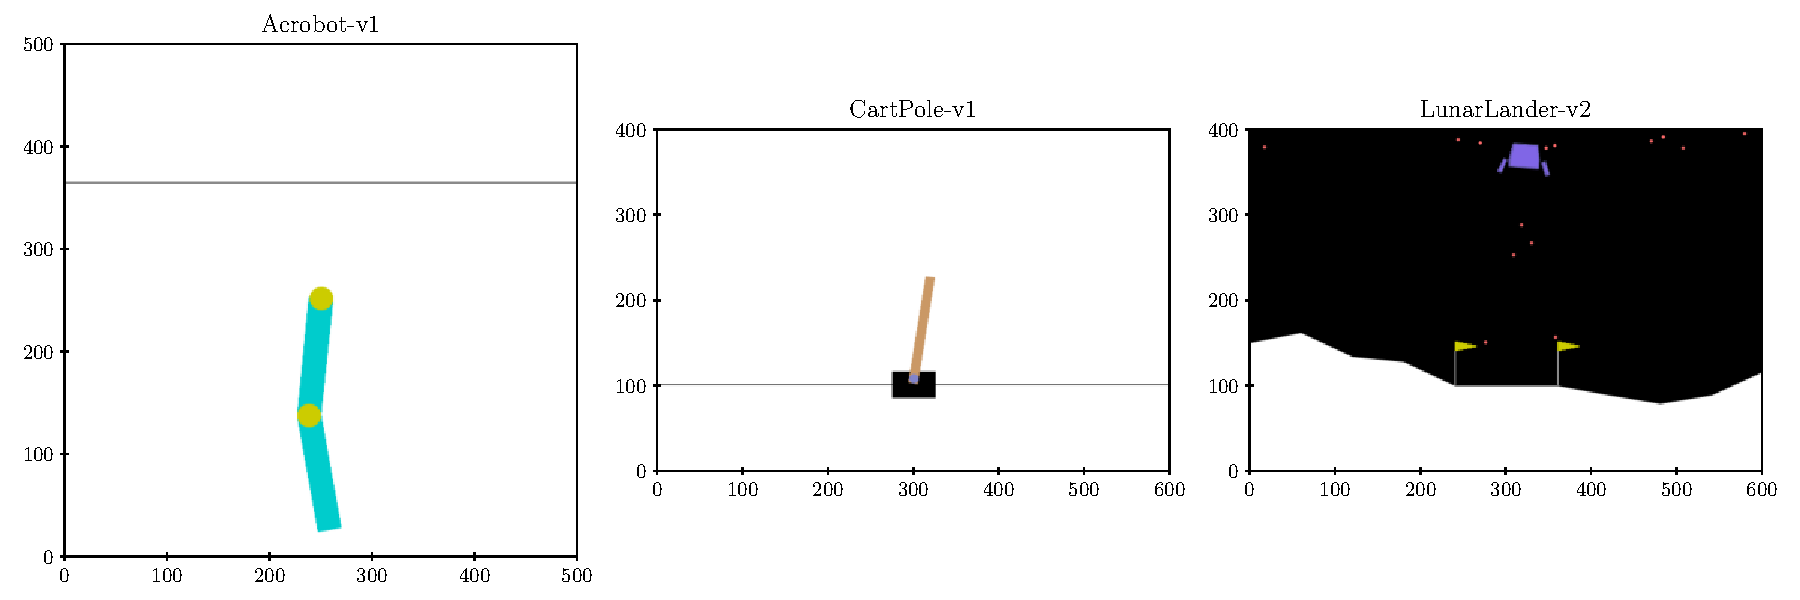
\includegraphics[width=\textwidth]{images/environments.pdf}
\caption{Example screenshots for each environment. From left to right: Acrobot, CartPole, LunarLander.}
\label{fig:environments}
\end{figure}

\subsubsection{Acrobot}
The Acrobot is a two-link under-actuated robot, an arm with the first joint fixed in place, and the joint between the two links actuated \cite{acrobot}.

The observation contains the values of the $\sin$ and $\cos$ of the two joints, and their respective angular velocities. The three possible actions are applying positive torque, negative torque, and no torque to the actuated joint. The objective is to swing the other end above the bar by an amount equal to the length of one of the links. The reward is $-1$ for each step taken and an episode ends if the robot either reaches the bar or takes the maximum number of allowed steps. An episode is considered successful if it reaches a reward threshold of $-100$ \cite{farama_gymnasium}.

A reward function that provides a fixed negative reward at each step, regardless of the state, is easy to design and pushes the agent to find its way to the target in the shortest possible amount of time. Conversely, the agent relies on the reward as a feedback on how good/bad the action taken is, and since the reward does not change, the agent may not have sufficient information to distinguish the good actions from the bad ones.

\subsubsection{CartPole}
The CartPole is a cart to which a rigid pole is hinged on its center. The cart moves on a frictionless track and the pole starts from an upright position \cite{cartpole}.

At each step, the available information about the environment is the cart position and linear velocity, and the pole angle and its angular velocity. The agent has no control on the pole, but it can push the cart left or right instead. Despite being discrete actions, the velocity is modeled depending on the angle of the pole. The reward is $+1$ for each step taken and the objective is to keep the pole upright for as long as possible. An episode terminates if the maximum score of $500$ is reached, if the cart goes beyond the edges of the frame, or if the pole is too tilted \cite{farama_gymnasium}.

Similar to \textit{Acrobot}, the CartPole agent receives a constant reward at each step taken, but this time it is a positive $+1$. Again, the agent cannot rely on the reward to gauge the optimality of its actions, but instead the implicit target is to keep the episode running for as long as possible.

\subsubsection{LunarLander} \label{subsubsec:lunar_lander}
The LunarLander environment is a rocket trajectory optimization problem. The lander has infinite fuel and it can either run the engines at full throttle or turn them off \cite{openai_gym}.

The observation provides information about the position of the lander in the space, the linear $x$ and $y$ velocities, its tilt, its angular velocity and whether or not each of the legs has touched the ground. The possible actions the lander can take are either be idle, or fire the engines (left, main or right respectively). The reward is modulated according to the distance from the landing pad, its speed and its tilt. An additional reward of $\pm 100$ is assigned after either landing safely or crashing \cite{farama_gymnasium}.

Since the reward function for the LunarLander provides a \textit{shaped reward}, the agent is able to learn faster and make quick adjustments to its policy since it receives immediate feedback for each action taken. A shaped reward function better informs the agent on its closeness to the target but, at the same time, it is more difficult to design, and it may be exploited in unexpected ways. For example, instead of learning to land safely (in which case it would receive maximum reward), the LunarLander agent may learn to hover just above the landing pad because in that state it also receives a reward close to the maximum.

\subsection{Loss and Parameter Optimization}
To represent how well the predicted values align with the target values, I use the \acrfull{mse}, which is the average of the squared difference between two values:

$$
\ell(x, y) = \bar{L}, \quad L = \{ l_1, \dots, l_N \}^\intercal, \quad l_n = (x_n - y_n)^2,
$$

where $N$ is the batch size, $x$ and $y$ are tensors of $n$ elements each.

The Adam optimizer takes care of adapting the learning rate to each network parameter individually. The parameters with more significant gradients are updated according to a smaller effective learning rate, while parameters with smaller gradients get a larger effective learning rate. Furthermore, Adam optionally adds weight decay as a regularization technique that penalizes large weights during training \cite{adam}, but in this case it is not used.

The optimizer updates the weights according to the following logic:

$$
\theta_t \leftarrow \theta_{t-1}  - \alpha \cdot \hat{m}_t / (\sqrt{\hat{b}_t} + \omega),
$$

where $\theta_t$ is the updated weight, $\theta_{t-1}$ is the current weight, $\alpha$ is the learning rate, $\hat{m}_t$ is the biased first moment estimate, $\hat{b}_t$ is the biased second raw moment estimate, and $\omega$ is a small constant for numerical stability \cite{adam}.

\subsection{Algorithm Hyperparameters}
Although different in the implementation from Stable-Baselines 3 \cite{sb3}, I choose to use the same hyperparameter names in most of the cases.

Optimal hyperparameters for \acrshort{dqn} are taken from \texttt{rl-baselines3-zoo} \cite{rl_zoo3}; the same set of hyperparameters is used for \acrshort{tqn}. Every episode rollout is capped at a maximum of $500$ steps.

\begin{table}[!htbp]
\caption{Hyperparameters used across all runs.}
\label{table:hyperparameters}
\centering
\begin{tabular}{@{} r c c c @{}}
\toprule
& \textbf{Acrobot-v1} & \textbf{CartPole-v1} & \textbf{LunarLander-v2} \\
\midrule
max steps                   & 100.000 &  50.000 & 100.000 \\
gradient clip               &         &    10.0 &         \\
accumulate gradient batches &         &       1 &         \\
batch size                  &     128 &      64 &     128 \\
learning rate               &  6.3e-4 &  2.3e-3 &  6.3e-4 \\
buffer size                 &  50.000 & 100.000 &  50.000 \\
learning starts             &       0 &   1.000 &       0 \\
tau                         &         &     1.0 &         \\
gamma                       &         &    0.99 &         \\
train frequency             &       4 &     256 &       4 \\
gradient steps              &         &       1 &         \\
target update interval      &     250 &      10 &     250 \\
exploration fraction        &    0.12 &    0.16 &    0.12 \\
epsilon max                 &         &     1.0 &         \\
epsilon min                 &     0.1 &    0.04 &     0.1 \\
\bottomrule
\end{tabular}
\end{table}

\begin{itemize}
    \item \textit{max steps}: total number of environment steps to train on;
    \item \textit{gradient clip}: maximum value for the gradient clipping of the network parameters;
    \item \textit{accumulate gradient batches}: gradient steps to take before updating the policy; 
    \item \textit{batch size}: minibatch size for each policy update;
    \item \textit{learning rate}: how much the policy weights should be updated w.r.t. the loss gradient;
    \item \textit{tau}: soft update coefficient, if $\tau = 1$ a hard update is performed instead;
    \item \textit{gamma}: discount factor;
    \item \textit{train frequency}: steps to perform between each policy update;
    \item \textit{target update interval}: environment steps to take between each target network update;
    \item \textit{exploration fraction}: fraction of entire training period over which the exploration rate is reduced; e.g. if the max steps are $100.000$ and the exploration fraction is $0.12$, $\epsilon$ linearly decreases from $\epsilon_{\max}$ to $\epsilon_{\min}$ during the first $12.000$ steps; 
    \item \textit{epsilon max}: exploration factor, initial probability of taking a random action;
    \item \textit{epsilon min}: exploration factor, final probability of taking a random action.
\end{itemize}

\subsection{Network Hyperparameters Tuning}
For the \acrshort{tqn}, I use a trial-and-error approach to find the best hyperparameters to make the network learn and converge. I only focus on tuning the parameters of the new network architecture; the default \texttt{nn.Transformer}\footnote{\url{https://pytorch.org/docs/stable/generated/torch.nn.Transformer.html}} parameters ($6$ encoder layers, $6$ decoder layers, and $2048$ units for each hidden layer) provided by PyTorch are, computationally-wise, prohibitively expensive.

As a first step, I progressively decrease the number of layers until it is possible to train the network on a consumer GPU. On the GPU worker I used for training, the default Transformer parameters grind the iterations to a halt, the computation time explodes from mere minutes to hours, with sudden crashes of the system as a result of out-of-memory errors. I end up fixing the size of the encoder and decoder components to $2$ layers each.

I then focus on the size of the hidden encoder/decoder layers. $2048$ units are too much for such a simple input, and they destabilize the network. The model is too complex and it starts performing poorly on new observations. A very large hidden layer is also prone to the exploding or vanishing gradient problem. For this reason, I set the units of each hidden layer to $256$. This proves to be sufficient for the network to converge.

Lastly, I investigate the impact of the number of heads in this multi-head attention model. Setting it to $1$ brings the worst results during training; this is expected because a single attention head is not enough to capture the different  relationships and the more complex dependencies within the data. Setting the number of attention heads equal to $2$ already bring better results, but empirically the best results come by setting them equal to the size of the observation, $4$, $6$ and $8$ depending on the environment.
